\section{Theorie}
\label{sec:theorie}
\subsection{Brechungsindex und Reflexion von Röntgenstrahlung}
In diesem Versuch trifft Röntgenstrahlung auf die im Labordiffraktormeter platzierte Probe.
Röntgenstrahlung ist eine elektromagnetische Welle mit Wellenlängen $\lambda < \SI{10}{\nano\metre}$.
Tritt Strahlung aus einem Vakuum $n_1 = 1$ (näherungsweise auch Luft) auf ein Medium ($n_2 = n \neq 1$), so wird die Brechung des Strahls durch den \textbf{Brechungsindex}
\begin{equation}
    n = 1 - \delta + \mathrm{i} \beta
    \label{eqn:brechungsindex}
\end{equation}
mit der Korrektur $\delta$ und Absorption $\beta$ beschrieben.
Der Realteil des Brechungsindex ist für Röntgenstrahlung kleiner als 1.
\\
Im folgenden Teil wird die \textbf{Reflexion} von Röntgenstrahlung auf einer homogenen Schicht (ideale Glätte und unendliche Dicke) betrachtet.
Wie in \autoref{fig:reflexion_homogen} schematisch dargestellt, trifft eine elektromagnetische Welle aus dem Vakuum $n_1=1$ unter dem Einfallswinkel $\alpha_i$, auf ein Medium $n = 1 - \delta + \mathrm{i} \beta$. ($A$)
Die Welle wird teilweise mit $\alpha_f = \alpha_i$, also Ausfallswinkel gleich Einfallswinkel reflektiert. ($B$)
Ein Teil wird unter dem Winkel $\alpha_t$ transmittiert und tritt somit in das Medium ein. ($C$)
\begin{figure}
    \centering
    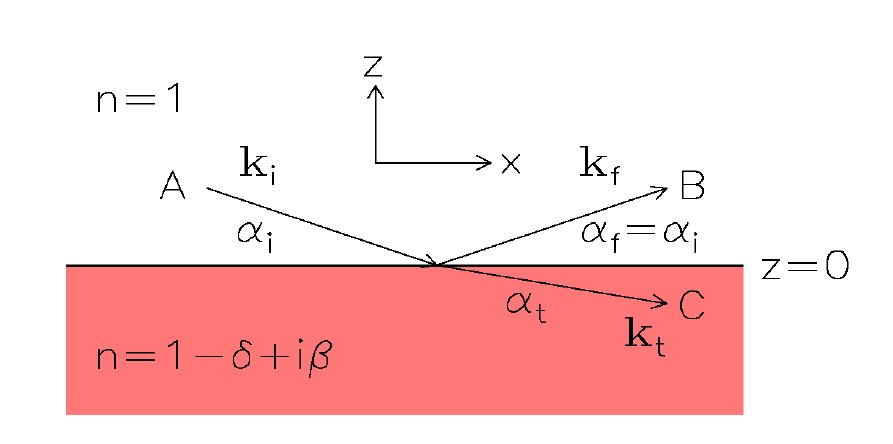
\includegraphics[width=0.8\textwidth]{content/data/reflexion_homogen.jpg}
    \caption{Brechung einer elektromagnetischen Welle auf einer homogenen Schicht.\cite[4]{alte_anleitung}}
    \label{fig:reflexion_homogen}
\end{figure}
\FloatBarrier
Zudem wird die Welle vollständig reflektiert, sobald der Einfallswinkel unter dem kritischen Winkel $\alpha_c$ mit
\begin{equation*}
    \cos \left ( \alpha_c \right ) = n
\end{equation*}
liegt.
Die Absorption liegt in dem Versuch in der Größenordnung $\beta \approx 10^{-7}$ und wird daher vernachlässigt.
Für den kritischen Winkel folgt näherungsweise
\begin{align}
    \alpha_c &\lambda \sqrt{\frac{r_e \rho}{\pi}} \label{eqn:kritisch_th}\\
    &= \approx \sqrt{2 \delta} \label{eqn:kritisch_exp} \, ,
\end{align}
wobei $\lambda$ die Wellenlänge der Röntgenstrahlung, $\rho$ die Elektronendichte des Materials und $r_e$ den Elektronenradius beschreibt.
Der transmittierte und reflektierte Anteil einer senkrecht zur Einfallsebene polarisierten Welle (s-polarisiert) wird durch die Fresnelschen Formeln beschrieben
\begin{align*}
    r &= \frac{2 n_1 \cos \left( \alpha_i \right)}{n_1 \cos \left( \alpha_i \right ) + n_2 \cos \left( \alpha_t \right )} \label{eqn:fresnel_r} \\
    t &= \frac{n_1 \cos \left( \alpha_i \right ) - n_2 \cos \left( \alpha_t \right )}{n_1 \cos \left( \alpha_i \right ) + n_2 \cos \left( \alpha_t \right )} \, . \label{eqn:fresnel_t}
\end{align*}
Der Transmissions- $t$ und Reflexionskoeffizient $r$ gilt bei Röntgenstrahlung näherungsweise auch für eine t-polarisierte Welle.
\\
Die Intensität einer Welle wird aus dem Betragsquadrat der Feldstärke berechnet. 
Daraus folgt für den Anteil reflektierter Strahlung zur einfallender Strahlung $R = |r^2|$.
Die Fresnelreflektivität $R_F$ kann für Röntgenstrahlung unter der Annahme $\alpha_i > 3 \alpha_c$ zu
\begin{equation}
    R_F \approx \left ( \frac{\alpha_c}{2 \alpha_i} \right )^4
    \label{eqn:fresnelreflektivitaet}
\end{equation}
approximiert werden.
\FloatBarrier

\subsection{Mehrschichtsysteme und der Parratt-Algorithmus}
In diesem Teil wird ein Körper mit \textbf{mehreren Schichten}, statt nur eine glatte Oberfläche betrachtet.
Betrachtet wird ein Polystyrolfilm auf Silizium, das auch in diesem Versuch verwendet wird.
\begin{figure}
    \centering
    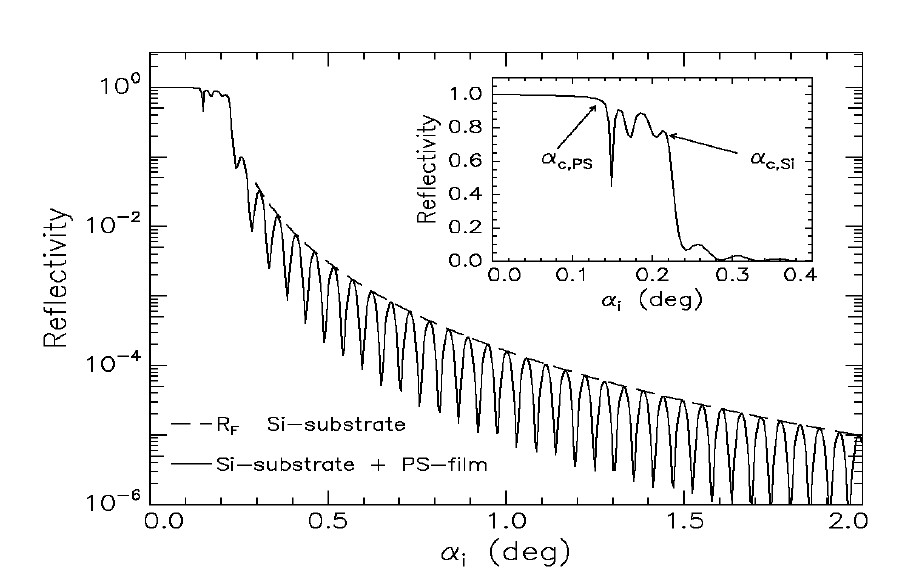
\includegraphics[width=0.8\textwidth]{content/data/reflektivitaet_plot.jpg}
    \caption{Die Reflektivität der Röntgenstrahlung in Abhängigkeit des Einfallswinkels $\alpha_i$.\cite[8]{alte_anleitung}}
    \label{fig:reflektivitaet_plot}
\end{figure}
In \autoref{fig:reflektivitaet_plot} ist die Röntgenreflektiviät in Abhängigkeit des Einfallswinkels $\alpha_i$ aufgetragen.
Der kleine Plot stellt den Bereich bis $\alpha_i = \SI{0.4}{\degree}$ hochauflösend da.
Es existieren zwei Grenzwinkel, der für die Polystyrolschicht $\alpha_\text{c,PS} = \SI{0.15}{\degree}$ und der des Siliziums $\alpha_\text{c,Si} = \SI{0.22}{\degree}$.
Zudem nimmt die Fresnelreflektivität (gestrichelte Linie) bei steigendem Einfallswinkel mit der vierten Potenz, wie nach \autoref{eqn:fresnelreflektivitaet} beschrieben ab.
\\
Die in das Medium eintreffende Welle wird an der Siliziumschicht teils reflektiert und trifft wieder auf das Vakuum und wird reflektiert.
Dieser Prozess wiederholt sich und die Wellen interferieren abhängig von der Phasendifferenz konstruktiv oder destruktiv.
Diese Oszillationen oder Modulationen sind in \autoref{fig:reflektivitaet_plot} zu sehen und werden als "Kiessig-Ringe" bezeichnet.
Beträgt der Gangunterschied $(2n+1) \cdot \frac{\lambda}{2}$ mit $n \in \mathbb{N}$, so kommt es zur destruktiven Interferenz und ein Minimum entsteht.
Ein Interferenzmaximum entsteht hingegen bei geraden Vielfachen von $\frac{\lambda}{2}$.
Die reflektierten Wellen im Medium interferieren konstruktiv miteinander.
\\
Der Schichtabstand bzw. die Dicke der Polystyrolschicht kann nach
\begin{equation}
    d = \frac{2\pi}{\Delta q_Z} \approx \frac{\lambda}{2 \Delta \alpha_i}
    \label{eqn:abstand_schicht}
\end{equation}
berechnet werden.
Wobei $\Delta q_Z$ die Differenz der z-Komponente des Wellenvektorübertrags und $\Delta \alpha_i$ die Differenz des Einfallswinkels zwischen zweier Minima darstellt.
\FloatBarrier

Zur Berechnung der Reflektivität in Mehrschichtsystemen wird der rekursiv-arbeitende \textbf{Parratt-Algorithmus} verwendet.
Betrachtet wird ein System mit $N-1$ Schichten, d.h. $N$ Grenzflächen.
Der Brechungsindex der $j$-ten Schicht mit einer Schichtdicke $d_j = z_{j-1} - z_j$ beträgt $n_j = 1 - \delta_j + \mathrm{i} \beta_j$.
Die einfallende Welle wird normiert und das Vakuum und genauso die unterste Schicht ($N+1$) werden als unendlich Dick angenommen.
Dies ist notwendig, damit die durch die unterste Grenzfläche ($z_N$) transmittierte Strahlung kein weiteres mal reflektiert wird und so ein Startwert $R_{N+1} = 0$ für die Rekursion feststeht.
Nun kann ausgehend von der untersten Schicht das Verhältnis der Amplitude der reflektierten zu der transmittierten Welle aufsteigend für jede Schicht berechnet werden.
Das Prinzip ist in \autoref{fig:parratt_alg} schematisch dargestellt.
\begin{figure}
    \centering
    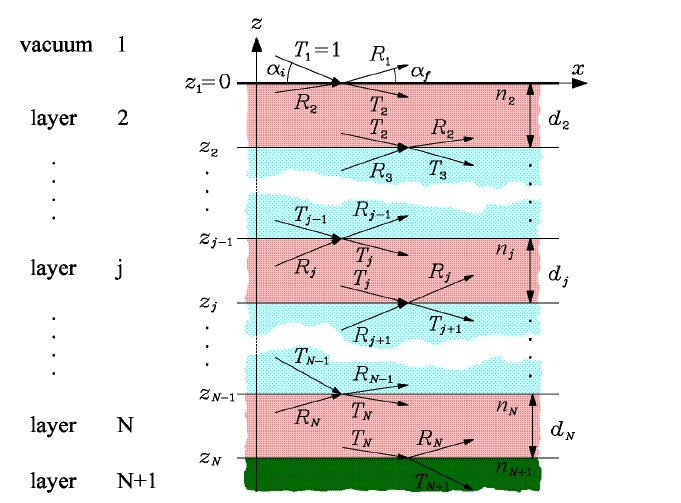
\includegraphics[width=0.8\textwidth]{content/data/parratt_algorithmus.jpg}
    \caption{Schematische Darstellung des Parratt-Algorithmus für ein System aus $N$ Schichten.\cite[10]{alte_anleitung}}
    \label{fig:parratt_alg}
\end{figure}
Für die $j$-te Grenzfläche wird das Verhältnis durch
\begin{equation*}
    X_j = \frac{R_j}{T_j} = \mathrm{e}^{-2\mathrm{i} k_{z,j} z_j} \cdot \frac{r_{j,j+1} + X_{j+1} \mathrm{e}^{2\mathrm{i} k_{z,j+1} z_j}}{1 + r_{j,j+1} X_{j+1} \mathrm{e}^{2\mathrm{i} k_{z,j+1} z_j}}
    \label{eqn:parratt_alg}
\end{equation*}
mit der Fresnelreflektivität der j-ten Grenzfläche $r_{j,j+1}$ und z-Komponente des Wellenvektors $k_{z,j}$
\begin{align*}
    r_{j,j+1} &= \frac{k_{z,j} - k_{z,j+1}}{k_{z,j} + k_{z,j+1}} \, ,\\
    k_{z,j} &= k \sqrt{ n_j^2 - \cos^2 \alpha_i} \, .
\end{align*}
\FloatBarrier

\subsection{Rauigkeit}
In der Realität existieren auf mikroskopischer Ebene keine idealen glatten Oberflächen.
Die Fresnelkoeffizienten müssen daher mithilfe der 'root-mean-square'-Rauigkeit (rms)
\begin{equation*}
    \sigma_j^2 = \int \left ( z - z_j \right )^2 P_j(z) \, \mathrm{d}z
    \label{eqn:rms}
\end{equation*}
angepasst werden.
Hierbei steht $P_j(z) \, \mathrm{d}z$ für die Wahrscheinlichkeit, dass die j-te Grenzfläche im Intervall $[z_j + z, z_j + z + \mathrm{d}z]$ liegt.
Die Wahrscheinlichkeitsverteilung $P_j(z)$ wird durch eine Gaußfunktion beschrieben.
Die Rechnung zum Parratt-Algorithmus mit den modifizierten Fresnelkoeffizienten
\begin{align*}
    \tilde{r}_{j,j+1} &= {r}_{j,j+1} \mathrm{e}^{-2 k_{z,j} k_{z,j+1} \sigma_j^2} \label{eqn:mod_fresnel_r} \\
    \tilde{t}_{j,j+1} &= {t}_{j,j+1} \mathrm{e}^{(k_{z,j} - k_{z,j+1})^2 \cdot \frac{\sigma_j^2}{2}} \label{eqn:mod_fresnel_t}
\end{align*}
funktioniert analog zu der für glatte Oberflächen, wie bereits oben beschrieben.
\FloatBarrier

\subsection{D8-Labordiffraktormeter}
\label{sec:diffraktometer}
Das Experiment zur Reflektivitätsmessung mit Röntgenstrahlung findet in einem D8-Labordiffraktormeter statt.
Die Röntgenröhre und der Detektor können in einer Kreisbewegung um den Probentisch gefahren werden.
Die Röntgenstrahlung wird in einer, wie in \autoref{fig:roentgenroehre} dargestellten Röntgenröhre erzeugt.
\begin{figure}
    \centering
    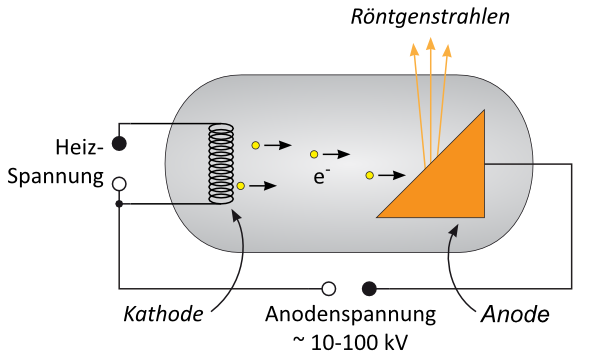
\includegraphics[width=0.6\textwidth]{content/data/roentgenroehre.png}
    \caption{Schematische Darstellung einer Röngenröhre zur Erzeugung von Röntgenstrahlung.\cite{uni_goettingen}}
    \label{fig:roentgenroehre}
\end{figure}
Elektronen werden aus einem Heizdraht durch den glühelektrischen Effekt emittiert und anschließend zur Anode hin beschleunigt.
Die Elektronen schlagen auf das Anodenmaterial ein und es entstehen drei Strahlungsarten:
\begin{itemize}
    \item Charakteristische Röntgenstrahlung
    \item Bremsstrahlung
    \item Lilienfeldstrahlung
\end{itemize}
Bremsstrahlung und Lilienfeldstrahlung werden der Vollständigkeit aufgeführt aber nicht weiter erläutert, da nur die char. Röntgenstrahlung verwendet wird.
Charakteristische Röntgenstrahlung entsteht, wenn ein Elektron ein anderes Elektron des Anodenmaterials aus seinem Platz in den inneren Atomschalen schlägt.
Ein freies Elektron oder ein Elektron aus einer höheren Schalen springen in die Leerstelle und es entsteht Röntgenstrahlung, mit einer Wellenlänge welche der Energiedifferenz entspricht.
\\
Der Röntgenstrahl trifft auf einen Göbelspiegel und wird gebündelt und monochromatisiert.
Der Strahl hat anschließend die Wellenlänge $\lambda = \SI{1.54}{\angstrom}$, welche der $K^\alpha$-Linie von Kupfer entspricht (daher werden weitere Strahlungsarten nicht beachtet).
Anschließend durchläuft der Röntgenstrahl einen Autoabsorber zur Abschwächung der Intensität und eine Blende um vorhandene Streuung auszublenden.
Mit einer weiteren Blende kann der Einfallswinkel $\alpha_i$ eingestellt werden.
Hinter der Probe befinden sich ebenfalls zwei Blenden, die zur Anpassung des Ausfallswinkel $\alpha_f$ dienen.
\newpage
\subsection{Geometriefaktor und Geometriewinkel}
\begin{wrapfigure}{r}{7.5cm}
    \caption{Schematische Darstellung des Strahlenverlaufs bei kleinem Einfallswinkel. Der Strahlendurchmesser ist größer als der der Probe.\cite[9]{anleitung}}\label{fig:geometrie}
    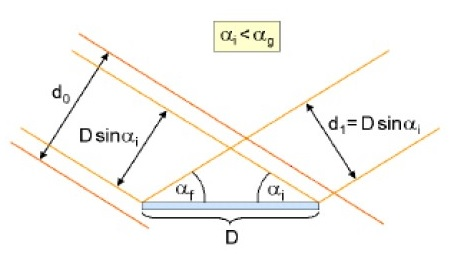
\includegraphics[width=7.5cm]{content/data/geometriefaktor.jpg}
\end{wrapfigure} 
%\begin{minipage}{0.5\textwidth}
%    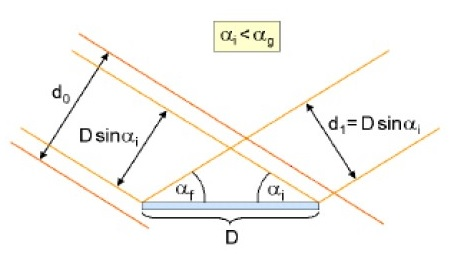
\includegraphics[width=\textwidth]{content/data/geometriefaktor.jpg}
%    \captionof{figure}{Schematische Darstellung des Strahlenverlaufs bei kleinem Einfallswinkel. Der Strahlendurchmesser ist größer als der der Probe.\cite[9]{anleitung}}
%    \label{fig:geometrie}
%\end{minipage}
%\begin{minipage}{0.5\textwidth}
%    Ab einem bestimmten Winkel, dem Geometriewinkel $\alpha_g$
%    \begin{equation}
%        \alpha_g = \sin \left ( \frac{d_0}{D} \right )
%        \label{eq:geometriewinkel}
%    \end{equation}
%    übersteigt der Durchmesser des Strahls den der Probenoberfläche $D$.
%    Dabei wird die Höhe des Strahls als $d_0$ bezeichnet.
%    Der Geometriefaktor für kleine Eintrittswinkel $\alpha_i < \alpha_g$ ist nach
%\end{minipage}
Bei kleineren Einfallswinkel $\alpha_i$ trifft der Röntgenstrahl (wie in \autoref{fig:geometrie} zusehen) nicht vollständig auf die Probe.
Ab einem bestimmten Winkel, dem Geometriewinkel $\alpha_g$
\begin{equation}
    \alpha_g = \sin \left ( \frac{d_0}{D} \right )
    \label{eq:geometriewinkel}
\end{equation}
übersteigt der Durchmesser des Strahls den der Probenoberfläche $D$.
Dabei wird die Höhe des Strahls als $d_0$ bezeichnet.
Der Geometriefaktor für kleine Eintrittswinkel $\alpha_i < \alpha_g$ ist nach
\begin{equation}
    G = \frac{D \sin \alpha_i}{d_0} \quad \text{für} \quad \alpha_i < \alpha_g
    \label{eqn:geometriefaktor}
\end{equation}
definiert.
Liegt der Eintrittswinkel des Strahls $\alpha_i$ über dem Geometriewinkel $\alpha_g$, so gilt $G=1$.
Der Geometriefaktor korrigiert die einfallende Intensität der Welle, die auf die Probe trifft.
%\begin{figure}
%    \centering
%    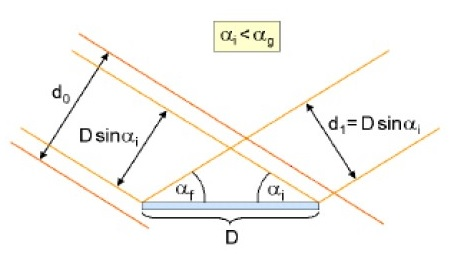
\includegraphics[width=0.7\textwidth]{content/data/geometriefaktor.jpg}
%    \caption{Schematische Darstellung des Strahlenverlaufs bei kleinem Einfallswinkel. Der Strahlendurchmesser ist größer als der der Probe.\cite[9]{anleitung}}
%    \label{fig:geometrie}
%\end{figure}